\documentclass{article}
\usepackage[utf8]{inputenc}
\usepackage[top=1in]{geometry}
\usepackage{graphicx}
\usepackage{booktabs}
\usepackage{tikz}
\usetikzlibrary{circuits.logic.US,positioning,calc} 
% Calligraphic fonts
\newcommand{\calA}{{\cal A}}
\newcommand{\calB}{{\cal B}}
\newcommand{\calC}{{\cal C}}
\newcommand{\calD}{{\cal D}}
\newcommand{\calE}{{\cal E}}
\newcommand{\calF}{{\cal F}}
\newcommand{\calG}{{\cal G}}
\newcommand{\calH}{{\cal H}}
\newcommand{\calI}{{\cal I}}
\newcommand{\calJ}{{\cal J}}
\newcommand{\calK}{{\cal K}}
\newcommand{\calL}{{\cal L}}
\newcommand{\calM}{{\cal M}}
\newcommand{\calN}{{\cal N}}
\newcommand{\calO}{{\cal O}}
\newcommand{\calP}{{\cal P}}
\newcommand{\calQ}{{\cal Q}}
\newcommand{\calR}{{\cal R}}
\newcommand{\calS}{{\cal S}}
\newcommand{\calT}{{\cal T}}
\newcommand{\calU}{{\cal U}}
\newcommand{\calV}{{\cal V}}
\newcommand{\calW}{{\cal W}}
\newcommand{\calX}{{\cal X}}
\newcommand{\calY}{{\cal Y}}
\newcommand{\calZ}{{\cal Z}}

% Sets:
\newcommand{\setA}{\textsf{A}}
\newcommand{\setB}{\textsf{B}}
\newcommand{\setC}{\textsf{C}}
\newcommand{\setD}{\textsf{D}}
\newcommand{\setE}{\textsf{E}}
\newcommand{\setF}{\textsf{F}}
\newcommand{\setG}{\textsf{G}}
\newcommand{\setH}{\textsf{H}}
\newcommand{\setI}{\textsf{I}}
\newcommand{\setJ}{\textsf{J}}
\newcommand{\setK}{\textsf{K}}
\newcommand{\setL}{\textsf{L}}
\newcommand{\setM}{\textsf{M}}
\newcommand{\setN}{\textsf{N}}
\newcommand{\setO}{\textsf{O}}
\newcommand{\setP}{\textsf{P}}
\newcommand{\setQ}{\textsf{Q}}
\newcommand{\setR}{\textsf{R}}
\newcommand{\setS}{\textsf{S}}
\newcommand{\setT}{\textsf{T}}
\newcommand{\setU}{\textsf{U}}
\newcommand{\setV}{\textsf{V}}
\newcommand{\setW}{\textsf{W}}
\newcommand{\setX}{\textsf{X}}
\newcommand{\setY}{\textsf{Y}}
\newcommand{\setZ}{\textsf{Z}}

% Vectors
\newcommand{\bfa}{\mathbf{a}}
\newcommand{\bfb}{\mathbf{b}}
\newcommand{\bfc}{\mathbf{c}}
\newcommand{\bfd}{\mathbf{d}}
\newcommand{\bfe}{\mathbf{e}}
\newcommand{\bff}{\mathbf{f}}
\newcommand{\bfg}{\mathbf{g}}
\newcommand{\bfh}{\mathbf{h}}
\newcommand{\bfi}{\mathbf{i}}
\newcommand{\bfj}{\mathbf{j}}
\newcommand{\bfk}{\mathbf{k}}
\newcommand{\bfl}{\mathbf{l}}
\newcommand{\bfm}{\mathbf{m}}
\newcommand{\bfn}{\mathbf{n}}
\newcommand{\bfo}{\mathbf{o}}
\newcommand{\bfp}{\mathbf{p}}
\newcommand{\bfq}{\mathbf{q}}
\newcommand{\bfr}{\mathbf{r}}
\newcommand{\bfs}{\mathbf{s}}
\newcommand{\bft}{\mathbf{t}}
\newcommand{\bfu}{\mathbf{u}}
\newcommand{\bfv}{\mathbf{v}}
\newcommand{\bfw}{\mathbf{w}}
\newcommand{\bfx}{\mathbf{x}}
\newcommand{\bfy}{\mathbf{y}}
\newcommand{\bfz}{\mathbf{z}}


\newcommand{\bfalpha}{\boldsymbol{\alpha}}
\newcommand{\bfbeta}{\boldsymbol{\beta}}
\newcommand{\bfgamma}{\boldsymbol{\gamma}}
\newcommand{\bfdelta}{\boldsymbol{\delta}}
\newcommand{\bfepsilon}{\boldsymbol{\epsilon}}
\newcommand{\bfzeta}{\boldsymbol{\zeta}}
\newcommand{\bfeta}{\boldsymbol{\eta}}
\newcommand{\bftheta}{\boldsymbol{\theta}}
\newcommand{\bfiota}{\boldsymbol{\iota}}
\newcommand{\bfkappa}{\boldsymbol{\kappa}}
\newcommand{\bflambda}{\boldsymbol{\lambda}}
\newcommand{\bfmu}{\boldsymbol{\mu}}
\newcommand{\bfnu}{\boldsymbol{\nu}}
\newcommand{\bfomicron}{\boldsymbol{\omicron}}
\newcommand{\bfpi}{\boldsymbol{\pi}}
\newcommand{\bfrho}{\boldsymbol{\rho}}
\newcommand{\bfsigma}{\boldsymbol{\sigma}}
\newcommand{\bftau}{\boldsymbol{\tau}}
\newcommand{\bfupsilon}{\boldsymbol{\upsilon}}
\newcommand{\bfphi}{\boldsymbol{\phi}}
\newcommand{\bfchi}{\boldsymbol{\chi}}
\newcommand{\bfpsi}{\boldsymbol{\psi}}
\newcommand{\bfomega}{\boldsymbol{\omega}}
\newcommand{\bfxi}{\boldsymbol{\xi}}
\newcommand{\bfell}{\boldsymbol{\ell}}

% Matrices
\newcommand{\bfA}{\mathbf{A}}
\newcommand{\bfB}{\mathbf{B}}
\newcommand{\bfC}{\mathbf{C}}
\newcommand{\bfD}{\mathbf{D}}
\newcommand{\bfE}{\mathbf{E}}
\newcommand{\bfF}{\mathbf{F}}
\newcommand{\bfG}{\mathbf{G}}
\newcommand{\bfH}{\mathbf{H}}
\newcommand{\bfI}{\mathbf{I}}
\newcommand{\bfJ}{\mathbf{J}}
\newcommand{\bfK}{\mathbf{K}}
\newcommand{\bfL}{\mathbf{L}}
\newcommand{\bfM}{\mathbf{M}}
\newcommand{\bfN}{\mathbf{N}}
\newcommand{\bfO}{\mathbf{O}}
\newcommand{\bfP}{\mathbf{P}}
\newcommand{\bfQ}{\mathbf{Q}}
\newcommand{\bfR}{\mathbf{R}}
\newcommand{\bfS}{\mathbf{S}}
\newcommand{\bfT}{\mathbf{T}}
\newcommand{\bfU}{\mathbf{U}}
\newcommand{\bfV}{\mathbf{V}}
\newcommand{\bfW}{\mathbf{W}}
\newcommand{\bfX}{\mathbf{X}}
\newcommand{\bfY}{\mathbf{Y}}
\newcommand{\bfZ}{\mathbf{Z}}


\newcommand{\bfGamma}{\boldsymbol{\Gamma}}
\newcommand{\bfDelta}{\boldsymbol{\Delta}}
\newcommand{\bfTheta}{\boldsymbol{\Theta}}
\newcommand{\bfLambda}{\boldsymbol{\Lambda}}
\newcommand{\bfPi}{\boldsymbol{\Pi}}
\newcommand{\bfSigma}{\boldsymbol{\Sigma}}
\newcommand{\bfUpsilon}{\boldsymbol{\Upsilon}}
\newcommand{\bfPhi}{\boldsymbol{\Phi}}
\newcommand{\bfPsi}{\boldsymbol{\Psi}}
\newcommand{\bfOmega}{\boldsymbol{\Omega}}


% Blackboard Bold:
\newcommand{\bbA}{\mathbb{A}}
\newcommand{\bbB}{\mathbb{B}}
\newcommand{\bbC}{\mathbb{C}}
\newcommand{\bbD}{\mathbb{D}}
\newcommand{\bbE}{\mathbb{E}}
\newcommand{\bbF}{\mathbb{F}}
\newcommand{\bbG}{\mathbb{G}}
\newcommand{\bbH}{\mathbb{H}}
\newcommand{\bbI}{\mathbb{I}}
\newcommand{\bbJ}{\mathbb{J}}
\newcommand{\bbK}{\mathbb{K}}
\newcommand{\bbL}{\mathbb{L}}
\newcommand{\bbM}{\mathbb{M}}
\newcommand{\bbN}{\mathbb{N}}
\newcommand{\bbO}{\mathbb{O}}
\newcommand{\bbP}{\mathbb{P}}
\newcommand{\bbQ}{\mathbb{Q}}
\newcommand{\bbR}{\mathbb{R}}
\newcommand{\bbS}{\mathbb{S}}
\newcommand{\bbT}{\mathbb{T}}
\newcommand{\bbU}{\mathbb{U}}
\newcommand{\bbV}{\mathbb{V}}
\newcommand{\bbW}{\mathbb{W}}
\newcommand{\bbX}{\mathbb{X}}
\newcommand{\bbY}{\mathbb{Y}}
\newcommand{\bbZ}{\mathbb{Z}}




\title{Homework 2}
\author{Max marks: 105}
\date{Due on September 18, 2023, before class. Please submit both in brightspace
  and in person in paper this time. Grading on paper is easier.}
\newtheorem{prob}{Problem}

\newcommand{\bx}{\bar{x}}
\newcommand{\by}{\bar{y}}
\newcommand{\bz}{\bar{z}}
\begin{document}

\maketitle

\begin{figure}
\begin{minipage}{0.5\linewidth}
\centering
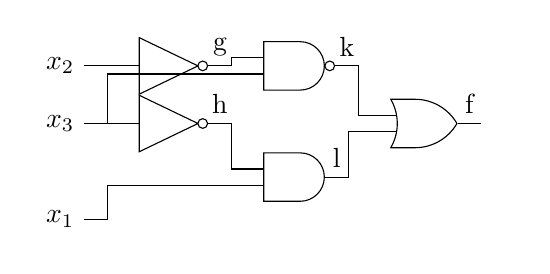
\begin{tikzpicture}[circuit logic US]
  \matrix[column sep=7mm]{
    \node (x2) {$x_2$}; & \node [not gate] (nx2) {};&  \node [nand gate] (x1nx2) {}; & \\
    \node (x3) {$x_3$}; & \node [not gate] (nx3) {};&  & \node [or gate] (f) {};\\
    & & \node [and gate] (x1nx3) {}; &  & \\
    \node (x1) {$x_1$}; & &  & \\
  };
  \draw (x2.east) -- ++(right:3mm) |- (nx2.input);
  \draw (nx2.output) to [edge label=g] ++(right:3mm) |- (x1nx2.input 1);

  \draw (x3.east) -- ++(right:3mm) |- (x1nx2.input 2);
  \draw (x3.east) -- ++(right:3mm) |- (nx3.input);
  \draw (nx3.output) to [edge label=h] ++(right:3mm) |- (x1nx3.input 1);

  \draw (x1.east) -- ++(right:3mm) |- (x1nx3.input 2);

  \draw (x1nx2.output) to [edge label=k] ++(right:3mm) |- (f.input 1);
  \draw (x1nx3.output) to [edge label=l] ++(right:3mm) |- (f.input 2);

  \draw (f.output) to [edge label=f] ++(right:3mm);

\end{tikzpicture}
\caption{A three-input circuit}
\label{fig:fig-2.24a}
\end{minipage}
\begin{minipage}{0.5\linewidth}
    \centering
    \begin{tabular}{ccc|c}
      \toprule
      $x_1$ & $x_2$ & $x_3$ & $f(x_1, x_2, x_3)$ \\
      \midrule
      0 & 0 & 0 & 0 \\
      0 & 0 & 1 & 1 \\
      0 & 1 & 0 & 1 \\
      0 & 1 & 1 & 0 \\
      1 & 0 & 0 & 1 \\
      1 & 0 & 1 & 1 \\
      1 & 1 & 0 & 1 \\
      1 & 1 & 1 & 0 \\
      \bottomrule
      \end{tabular}
    \caption{A three-variable function}
    \label{fig:fig-2.23}
\end{minipage}
\end{figure}

\begin{prob}
  Consider the circuit in Figure~\ref{fig:fig-2.24a}. Write the circuit as:
  \begin{enumerate}
    \item Boolean expression [5 marks]
    \item Truth table [10 marks]
    \item Venn diagram. [5 marks]
  \end{enumerate} (Total 20 marks)
\end{prob}

\begin{prob}
Represent the function in Figure~\ref{fig:fig-2.23} in the form of a 
\begin{enumerate}
  \item Venn diagram [5 marks]
  \item Boolean expression [5 marks]
  \item ANSI symbol network [5 marks]
  \item Timing diagram [5 marks]
\end{enumerate}
    Also, find its minimal sum-of-products form [5 marks].
    (Total 25 marks).
\end{prob}

\begin{prob}
Use algebraic manipulation to simplify the function $f = x_1x_3 + x_1x_2 + \bx_1 \bx_2 x_3 + \bx_1 \bx_2 \bx_3$. If the function is already in its simplest form, say so. [10 marks]
\end{prob}

\begin{prob}
Use algebraic manipulation to simplify the function $f = x_1 x_2\bx_3 + x_1\bx_2x_4 + x_1\bx_2 x_3\bx_4$. If the function is already in its simplest form, say so. [10 marks]
\end{prob}

\begin{prob}
Use algebraic manipulation to prove that $(x+y)\cdot(x+\bar{y}) = x$. [10 marks].
\end{prob}

\begin{prob}
Determine whether or not the following expressions are valid, i.e., whether the
left- and right-hand sides represent the same function.
[10 marks]
\begin{enumerate}
    \item $x_1 \bx_3 + x_2 x_3 + \bx_2 \bx_3 = (\bx_1 + \bx_2 + x_3)(x_1 + x_2 + \bx_3)(\bx_1 + x_2 + \bx_3)$
    \item $(x_1 + x_3)(\bx_1 + \bx_2 + \bx_3)(\bx_1 + x_2) = (x_1 + x_2)(x_2 + x_3)(\bx_1 + \bx_3)$
\end{enumerate}
\end{prob}

\begin{prob}
Design the simplest sum-of-products circuit that implements the function $f (x_1
, x_2 , x_3, x_4 ) = \sum m(3, 4, 6, 7, 8)$.[10 marks]
\end{prob}

\begin{prob}
Design the simplest product-of-sums circuit that implements the function $f (x_1 , x_2 , x_3 ) = \prod M (0, 2, 5, 6)$.[10 marks]
\end{prob}


%\bibliography{main}
%\bibliographystyle{plain}
\end{document}
